\chapter{Motivation} \label{cpt-motivation}


Ever since the early days of computer graphics, both hard- and software have rapidly evolved
alongside the creative and challenging use cases provided by developers, scientists and others.
Many technical increments relied on innovation, especially the advent of new capable hardware.
One example is the \ac{GPU} itself, which is now considered the heart of modern graphics 
processing and is widely used in fields like science, artificial intelligence, games, and pretty 
much all graphics related applications. Before 1995, there already had been a lot of iterations 
on specialized graphics hardware, often focused on video formatting or color output operations
(\cite{Singer2023}).

The first graphics cards were specialized chips either used for video encoding and decoding
or expensive hardware targeted for large companies, which arised during the early stages 
of "3D consumer graphics" (\cite{Singer2023}). Dedicated and affordable \ac{GPU}s for consumer 
\ac{PC}s had their large breakthrough during the 1990's. In 1999, NVidia introduced their 
first consumer graphics chip, the \emph{NVIDIA GeForce 256}, which was used for efficient 
transformations and lighting (\cite{Fenno2024}). Back then, this new hardware created a multitude 
of new possibilities. 
Although it was mostly used for graphics processing - hence the name - nowadays, \ac{GPU}s
are used in a much more general way than in [@TODO: insert year of GPU advent]. Both the 
technical complexity and the fields of application have tremendously increased. Today, a 
\ac{GPU} is often also reffered to as a \ac{GPGPU} instead, because of its evolution towards 
a multi-purpose tool. \\

\noindent
Nevertheless, \ac{GPU} architecture is still under a strong influence of the entertainment 
industry, first and foremost the games industry. Some of the latest changes to \ac{GPU} 
hardware and \ac{API} design correlates to the ongoing demand for higher output resolutions, 
higher geometric density or additionaly technology for \emph{Deep Learning} algorithms. 
To provide more context for how we made use of some of the more modern features of \ac{GPU}s 
we will give a brief overview over the trends in computer graphics over the past decades, and 
especially the last years.


\section{The Rise Of The GPU}

Before the integration of specialized hardware, games like Wolfenstein 3D or the original Doom made use of 
\ac{CPU} Rasterization, with all rendering operations executed sequentially by the \ac{CPU} [@TODO: check games and facts].
[@TODO: Check if rendering ops were ALL on CPU]
Therefore, a higher poly count usually led to lower framerates.

\subsection{Rendering Pipeline}

With the first \ac{GPU} available to larger audiences, games were able to add more and more 
detail into their 3D environment. The heavily parallelized transformations allowed for a lot 
more triangles in games and the hardware accelerated lighting computations which made for 
even more realistic lighting throughout the rendered scene. Having a dedicated hardware for 
highly demanding tasks started a new era of computer graphics. One significant advantage: 
The \ac{GPU} could operate on a large amount of data while not stalling the \ac{CPU} (\cite{Fenno2024}).\\

\noindent 
This new approach of "outsourcing" specific operations quickly became the standard procedure and 
lead to a standardized rendering pipeline. 



\subsection{Deferred Rendering}



\subsection{GPU Driven Rendering}


\section{Hier kommt meine Motivation und Überleitung zur Forschungsfrage}

The latest innovations in computer graphics have been developing in different directions,
one of them being \ac{GPU} Driven Rendering. Minimizing dependencies between \ac{CPU} and \ac{GPU} 
has been an effort for the last decade. Many of the novel approaches which have been developed 
over the years are visible in the latest technology. But there are still plenty of use cases 
which are not yet living up to there full potential, considering modern hard- and software solutions.\\

\noindent
One of those use cases is Voxel Rendering. Although there are ongoing efforts to improve voxel 
rendering performance, we believe that new innovations can be applied to this field of computer 
graphics. To highlight the possible improvements, one can consider different applications of 
voxel rendering. 

\subsection{Rasterized Voxel Rendering}

The basic approach to rendering voxels is using the traditional Rasterized Rendering Pipeline.
One of the most popular games of all time, Minecraft [@TODO: reference] uses this approach to 
render thousands of cube shaped voxels on screen. Minecraft also makes use of different rendering 
optimizations to optimize frame times. This approach is straight forward in concept and can be 
implemented for existing \ac{API}s, making use of hardware acceleration, i.e. the \ac{GPU}.
The voxel representation allows for easy computations since geometry is laid out in a regular grid.
Lighting calculations, as well as phyisics operations, can be further optimized to be even more 
efficient. The most significant advantage is the ability to dynamically enable or disable voxels 
within the grid. Or, in general, to update voxels and their corresponding data efficiently.\\

\noindent
Since voxels are regular shapes, they can be easily created on the \ac{GPU} as supposed to being 
sent over the PCI Express port. 

[@TODO: Write more!]


\subsection{Ray Traced Voxel Rendering}

[@TODO: Add citations for all examples]
A rather common approach to visualization of voxels in 3D space is \emph{Ray Tracing}. When using 
Ray Tracing, it is essential to consider different acceleration strategies. The regular 
and memory efficient encoding of voxels allows for efficient tracing against the geometry. 
Another acceleration technique is to use \ac{BSP} Trees or similar spatial algorithms which store 
information about the layout of geometry in space. This can help discard parts of a scene which are 
not of interest for the computational process or (e.g. using an \emph{Octree} data structure) store 
more detailed data in one part of a scene and keep the data resolution low in parts, where (almost) 
no geometry is present. Geometry doesn't even have to be present, since voxels can be stored 
as a bit value, storing (1) either a voxel within a given part of the scene (e.g. in a regular grid),
or keeping the bit clear (0) if no voxel is present at the given location. 
Ray Traced approaches not always make use of the volumetric nature of voxel scenes, but often generate 
voxels only where necessary for faster traversal. A \ac{SVO} only stores octree nodes, and therefore voxel 
data, where there is actually data present, skipping paths down the hierarchical structure which are not 
contributing to the final scene data. Still, Ray Tracing is a very expensive operation, depending on the 
data that is being computed during each ray sample. That means that voxel resolutions have to be adapted 
according to the use case. [@TODO: check that these informations are not meant for related work].

\subsection{Voxel based physics}

\begin{figure}[h]
    \centering
    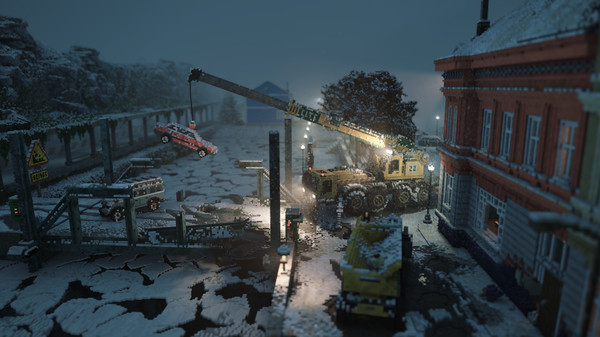
\includegraphics[width=\linewidth]{images/graphics/teardown.jpg}
    \caption{The voxel based sandbox Teardown (2022) by Tuxedo Labs.}
    \label{fig:teardown}
\end{figure}

Tuxedo Labs \emph{Teardown} (figure \ref{fig:teardown}) uses ray traced lighting which is affordable due 
to the voxel scene representation. [@TODO: Check Teardown ray tracing]
Additionally, it makes use of highly dynamic physics operation which are relatively efficient using the voxel 
representation. In their base layout, cubical voxels are \ac{AABB}es which allows for trivial collision tests.
When rotated around any axis, they are still oriented bounding boxes, making collision tests more expensive,
but still rather efficient. These characteristics make voxels excellent candidates for dynamic physics 
calculations. Also, storing voxels in a spatial container helps keep collision checks to a minimum. \\

\noindent
In the next chapter we will focus on the first use case, the Rasterized Voxel Rendering. We belive that this 
technique can benefit the most from advances in rendering technology.
With most of the latest improvements of graphics hard- and software, the capabilities to process mesh data 
and compute a rasterized image got better and better. Even the graphics hardware vendors efforts to enable 
real time ray traced lighting, shadows, reflections and ambient occlusion is applied within the rasterized 
pipeline and therefore relies on improvements to said paipeline over the last years. \\
We will first lay out a technical foundation in chapter \ref{cpt-technical-background} before discussing 
related work on which our approach relies on in chapter \ref{cpt-related-work}.







- Spectrum between CPU computation and GPU computation. 
CPU <-----------> GPU

- Mesh-Shading pipeline as new standard 

- Poses question, can mesh shading further optimize voxel rendering?

- Voxel Rendering

- Better geometry creation (in contrast to Geometry Shader)
- Optimized occlusion culling using per-meshlet OC
